%!TEX root =  tfg.tex
\chapter{Manual de usuario}

\begin{quotation}[Novelist]{Ernest Hemingway (1899--1961)}
The good parts of a book may be only something a writer is lucky enough to overhear or it may be the wreck of his whole damn life -- and one is as good as the other.
\end{quotation}

\begin{abstract}
Este capítulo constituye el manual de usuario de la aplicación, cuyo objetivo es servir de guía detallada para que los usuarios puedan comprender y utilizar la interfaz gráfica y todas las funcionalidades del sistema.

En la Sección \ref{sec:pantalla_inicial}, se explica la disposición y uso de la pantalla inicial.
En la Sección \ref{sec:registro}, se expone el proceso necesario para registrarse e iniciar sesión en el sistema.
En la Sección \ref{sec:amistad}, se presenta el funcionamiento de la ventana de amistades.
En la Sección \ref{sec:listado_salas}, se detalla la navegación por el listado de salas disponibles.
En la Sección \ref{sec:sala}, se describe el comportamiento y las opciones de una sala de espera.
En la Sección \ref{sec:partida}, se explica la interfaz principal del juego y las acciones de turno.
Finalmente, en la Sección \ref{sec:fin_partida}, se justifica el proceso que tiene lugar al concluir una era y al finalizar la partida completa.
\end{abstract}

\section{Pantalla Inicial}
\label{sec:pantalla_inicial}

\begin{figure}[H]
\begin{center}
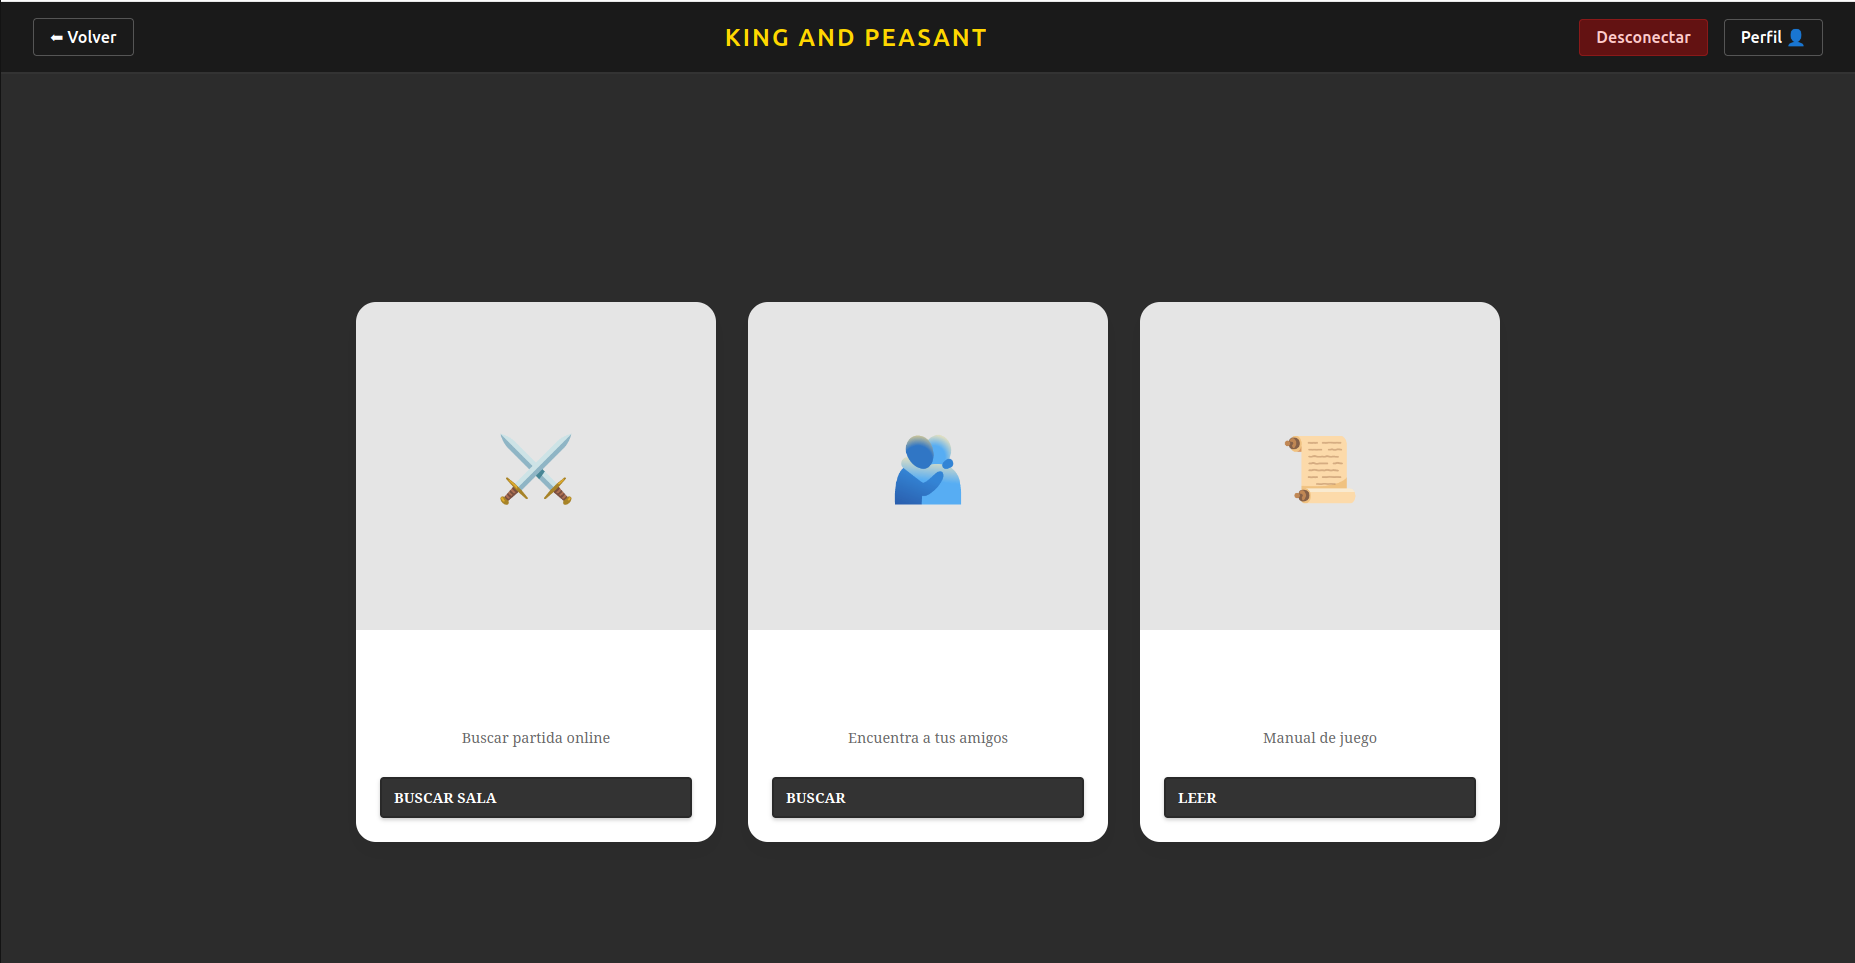
\includegraphics[width=\textwidth]{figures/manual/Pantalla Inicio.png}
\caption{Pantalla Inicio}
\label{fig:Manual01}
\end{center}
\end{figure}

Como se puede observar en la Figura \ref{fig:Manual01}, al entrar en la aplicación nos encontramos con la pantalla de inicio. Esta pantalla actúa como el eje central de navegación y presenta tres grandes paneles centrales que nos dan acceso a las distintas funcionalidades principales: ``Buscar partida online'' (para ir al listado de salas), ``Encuentra a tus amigos'' (para gestionar el aspecto social de la cuenta) y ``Manual de juego'' (para consultar las reglas).

Además, en la barra de navegación superior derecha, disponemos de botones rápidos para acceder a nuestro ``Perfil'' o para ``Desconectar'' la cuenta actual. En caso, de que no se haya iniciado sesión, aparecerán dos botones, uno para acceder al ``Registro'' y otro para acceder a la pantalla de ``Inicio de Sesión''. Para comenzar a utilizar todas estas opciones, el sistema nos requerirá haber iniciado sesión previamente.

\section{Registro/Inicio de Sesión}
\label{sec:registro}

Para acceder a las funcionalidades de la aplicación, el usuario debe identificarse. Si somos nuevos jugadores, debemos registrarnos desplegando el formulario de creación de cuenta (Figura \ref{fig:Manual02}). En este modal, titulado \textit{New Lord}, se nos solicitará introducir un nombre de usuario (\textit{Name}), un correo electrónico válido (\textit{Email}) y una contraseña segura (\textit{Password}). Tras completarlos, pulsaremos el botón rojo de \textit{Register}.

\begin{figure}[H]
\begin{center}
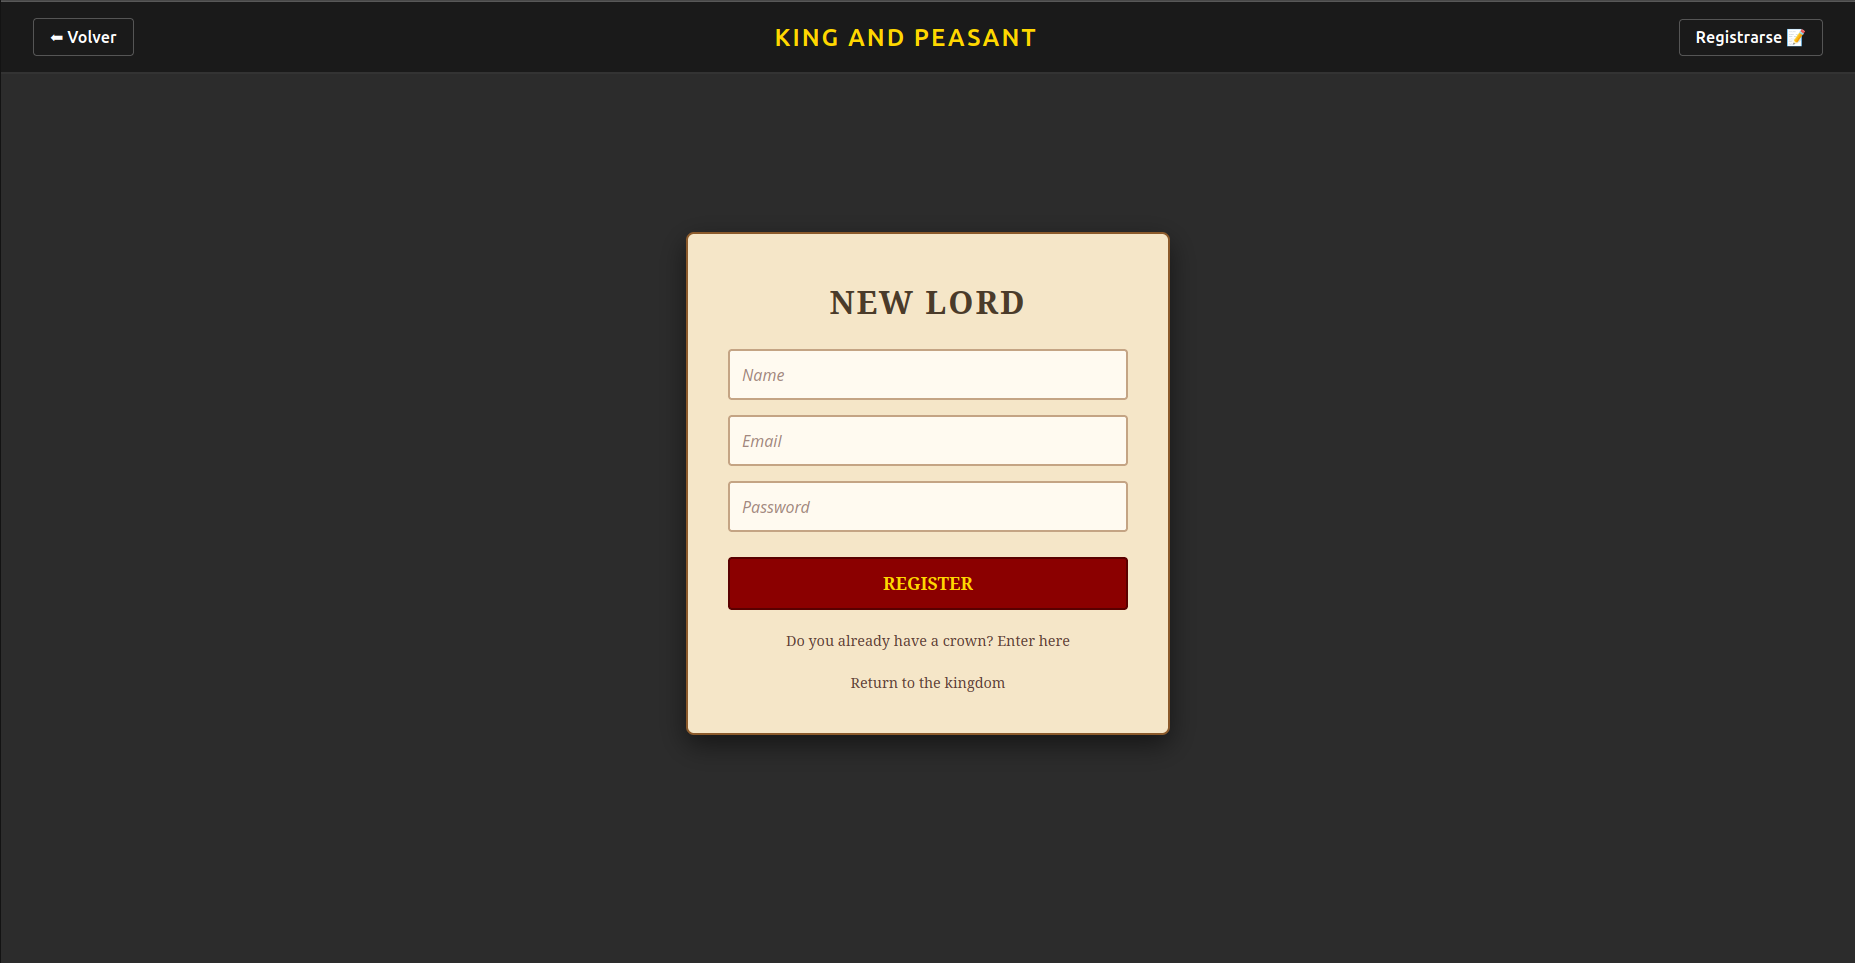
\includegraphics[width=\textwidth]{figures/manual/Registro.png}
\caption{Pantalla de Registro}
\label{fig:Manual02}
\end{center}
\end{figure}

Una vez registrados, o si ya poseíamos una cuenta previamente, podemos iniciar sesión desde la pantalla de \textit{Login} (Figura \ref{fig:Manual03}). Aquí simplemente introduciremos nuestro correo electrónico y contraseña en los campos habilitados y pulsaremos sobre el botón de confirmación. Ambas pantallas cuentan con enlaces inferiores para alternar ágilmente entre el inicio de sesión y el registro, así como para regresar a la vista principal.

\begin{figure}[H]
\begin{center}
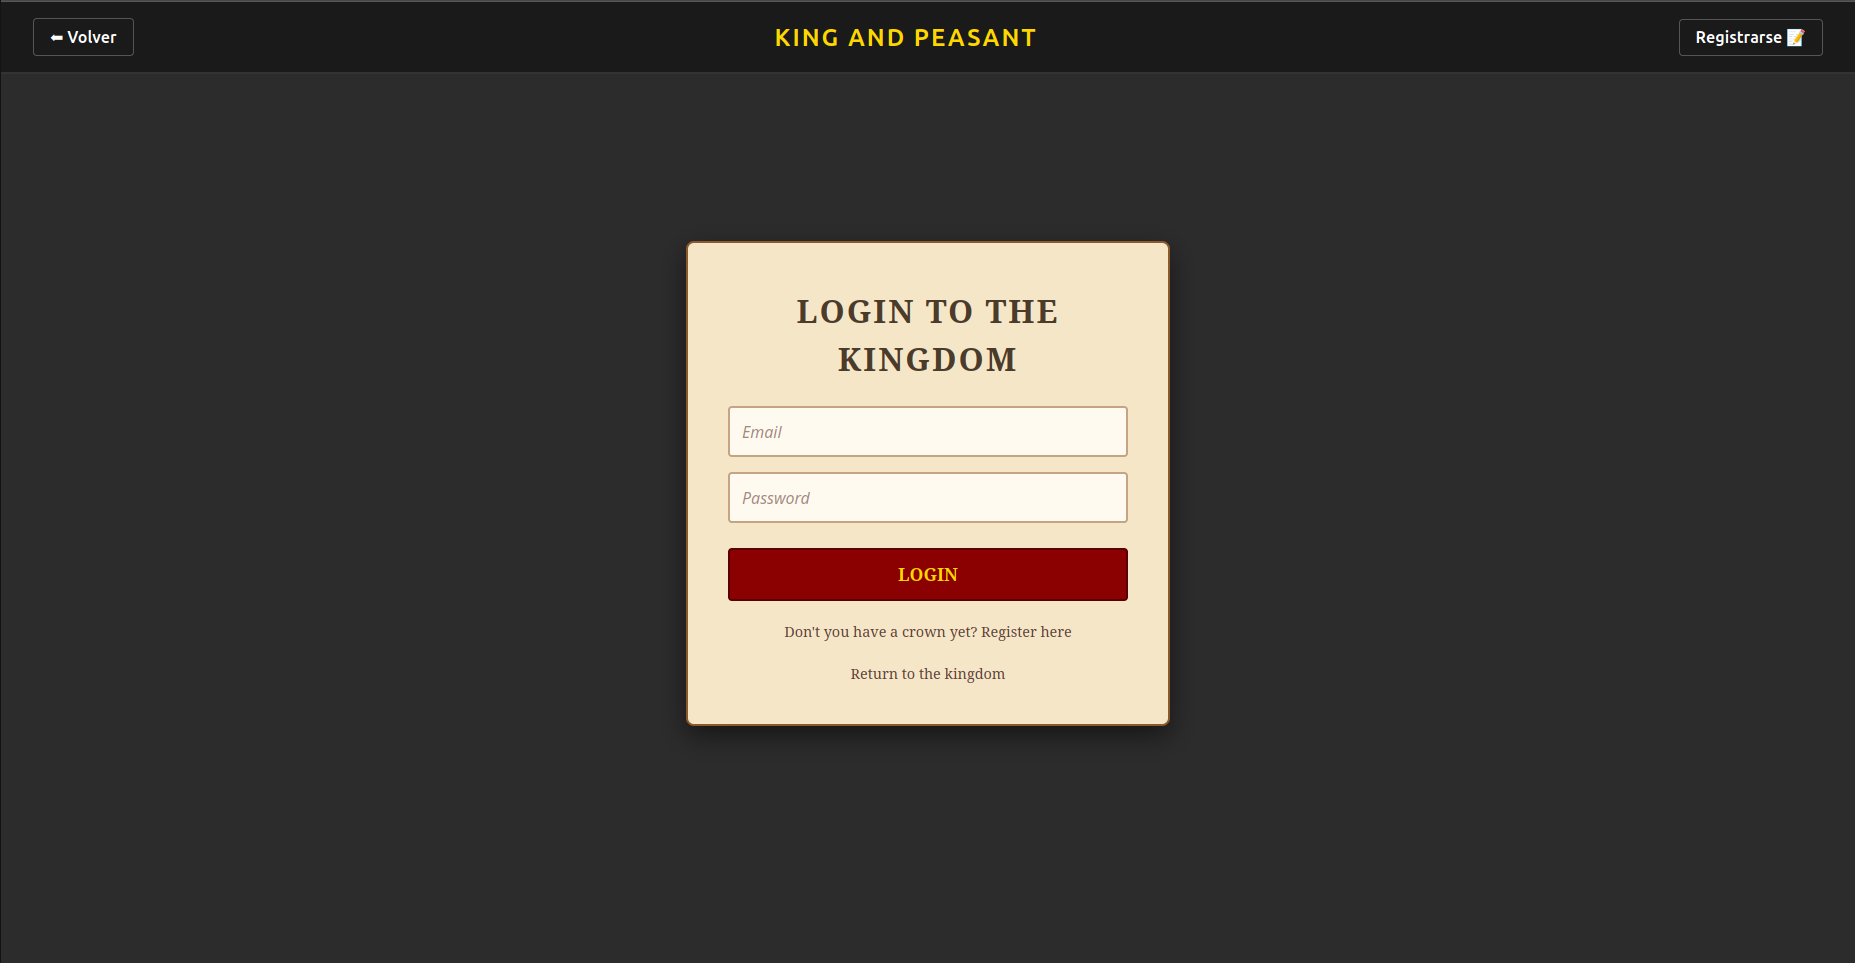
\includegraphics[width=\textwidth]{figures/manual/Login.png}
\caption{Pantalla de Inicio de Sesión}
\label{fig:Manual03}
\end{center}
\end{figure}

\section{Amistad}
\label{sec:amistad}

\begin{figure}[H]
\begin{center}
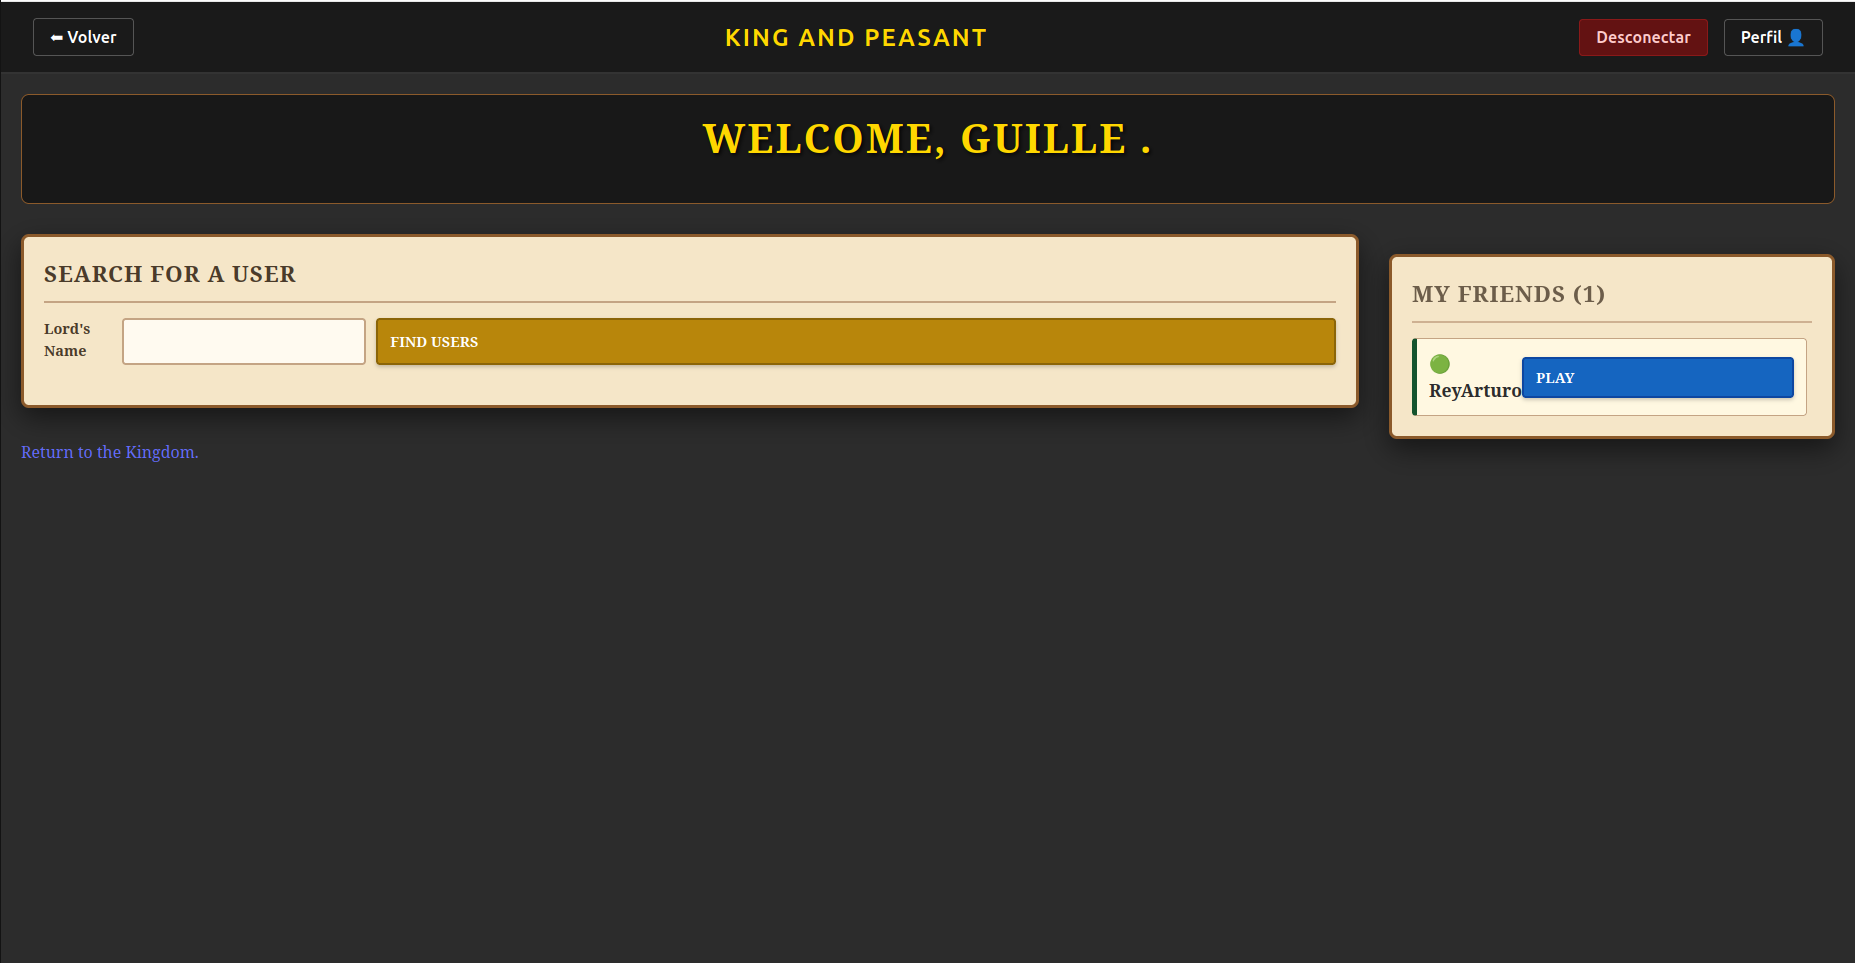
\includegraphics[width=\textwidth]{figures/manual/Amistad.png}
\caption{Pantalla de Amistad}
\label{fig:Manual10}
\end{center}
\end{figure}

La Figura \ref{fig:Manual10} ilustra la pantalla de Amistad, diseñada para la interacción con otros jugadores. La interfaz se divide en dos bloques principales. En la parte izquierda (\textit{Search for a user}), disponemos de un cuadro de texto para introducir el nombre de otro usuario y buscarlo mediante el botón \textit{Find Users}, lo que nos permite enviar nuevas peticiones de amistad.

En la parte derecha de la pantalla encontramos el panel \textit{My Friends}, que lista todos los amigos que ya tenemos agregados. Este listado muestra el nombre de cada amigo junto con un indicador visual (como un círculo verde) que señala su estado de conexión. Además, incluye un botón directo de \textit{Play} para invitar rápidamente a ese amigo a una partida sin necesidad de buscar su sala manualmente.

\section{Listado de Salas}
\label{sec:listado_salas}

\begin{figure}[H]
\begin{center}
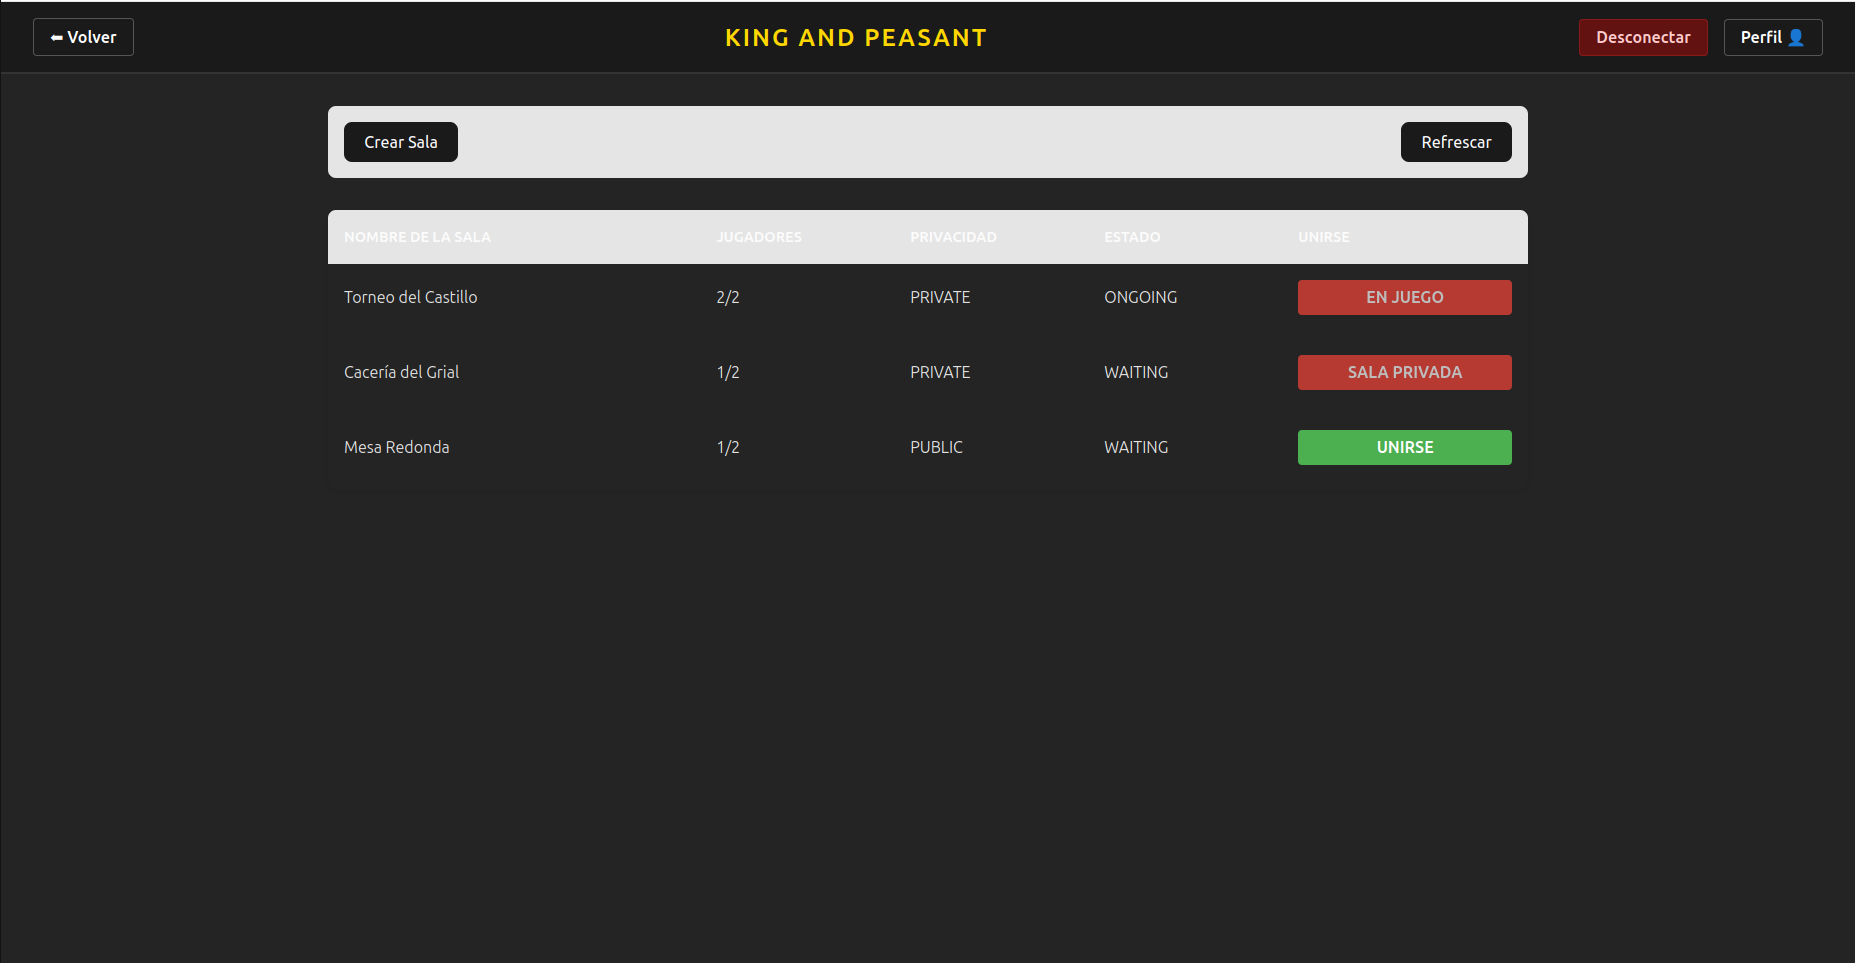
\includegraphics[width=\textwidth]{figures/manual/Listado de Salas.png}
\caption{Pantalla de Listado de Salas}
\label{fig:Manual04}
\end{center}
\end{figure}

Como se aprecia en la Figura \ref{fig:Manual04}, la pantalla de Listado de Salas presenta una tabla que recopila todas las partidas creadas en el servidor. La tabla está estructurada en cinco columnas informativas: Nombre de la Sala, Jugadores (mostrando el aforo actual frente al máximo, ej. 1/2), Privacidad (Pública o Privada), Estado (Esperando o En Juego) y una columna final de acción para Unirse. En la parte superior de la tabla contamos con un botón negro para \textit{Refrescar} la lista en tiempo real.

Desde esta interfaz podemos realizar las siguientes acciones:

\subsection{Crear Sala}

\begin{figure}[H]
\begin{center}
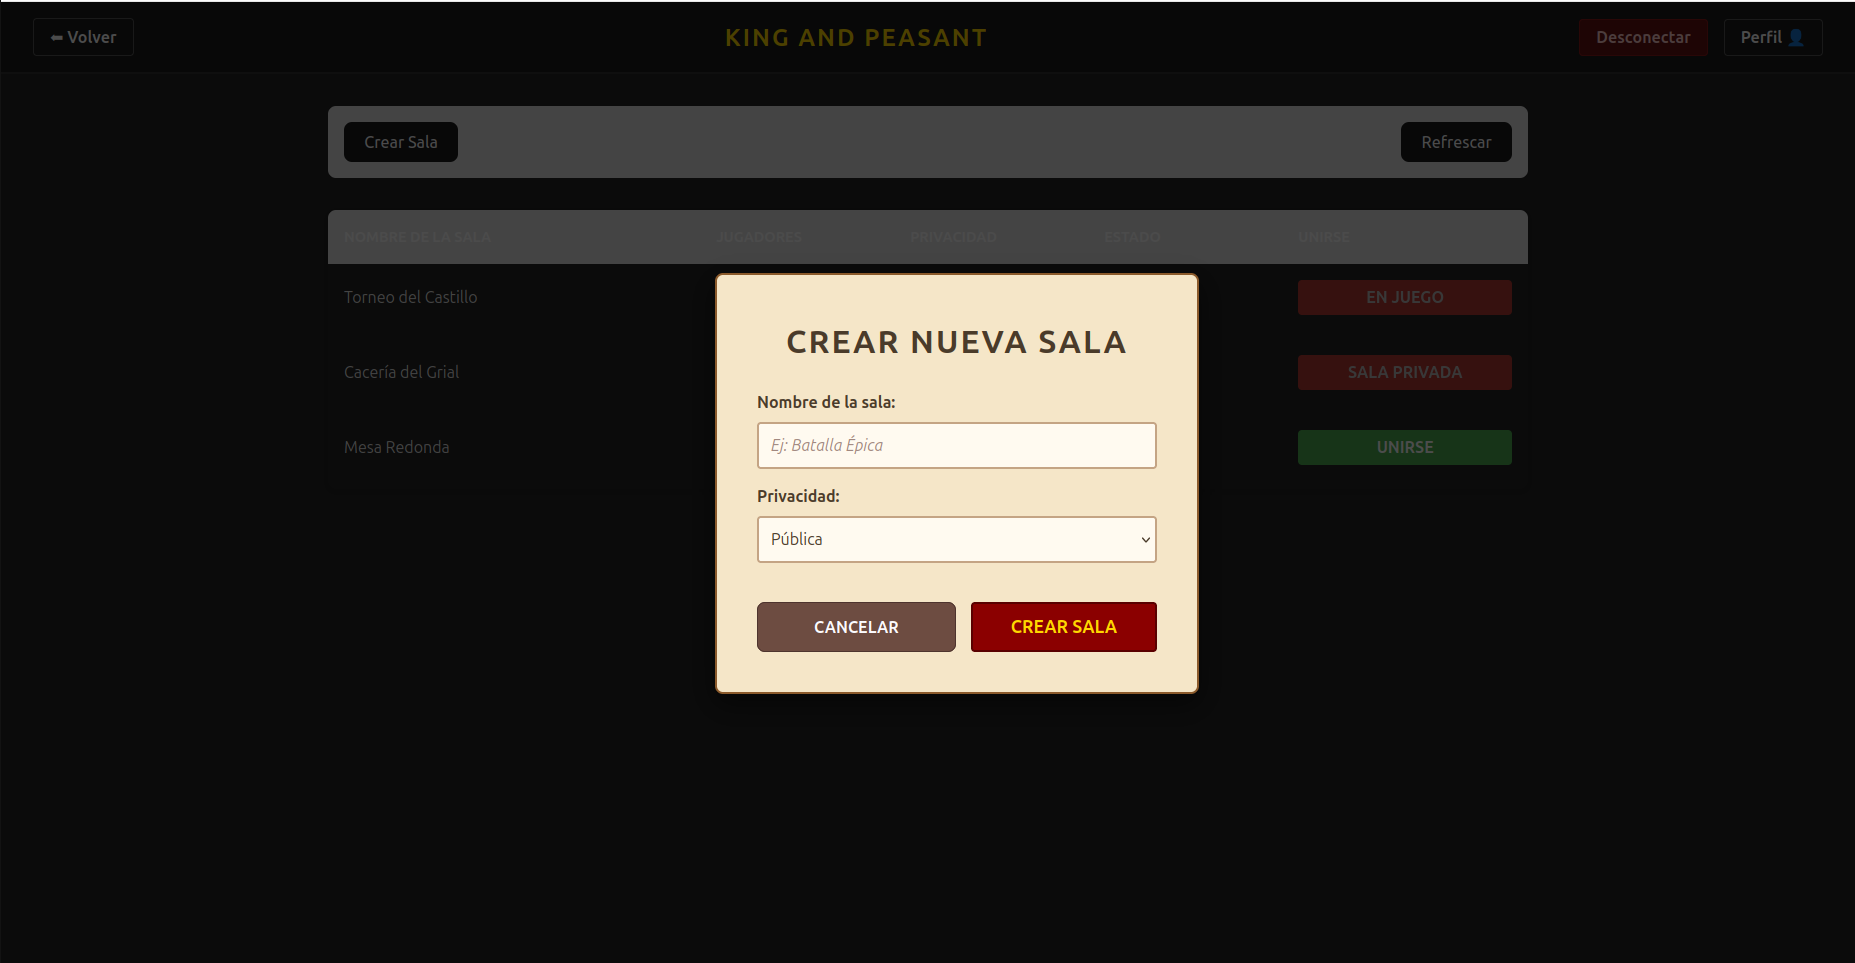
\includegraphics[width=\textwidth]{figures/manual/Crear Sala.png}
\caption{Pantalla de Listado de Salas: Crear Sala}
\label{fig:Manual05}
\end{center}
\end{figure}

Al pulsar el botón negro de \textit{Crear Sala} situado en la esquina superior izquierda, se desplegará el cuadro de diálogo mostrado en la Figura \ref{fig:Manual05}. En este formulario deberemos asignar un nombre descriptivo a nuestra sala y utilizar el menú desplegable para establecer su privacidad (determinando si cualquiera puede entrar o si requiere invitación).

\subsection{Unirse a una Sala}

Si no nos encontramos actualmente vinculados a ninguna sala, los botones de la columna derecha de la tabla estarán habilitados. Podremos pulsar el botón verde de \textit{Unirse} en aquellas salas públicas que se encuentren en estado de espera (\textit{Waiting}) y que no hayan alcanzado su límite de jugadores.

\subsection{Volver a la sala}

\begin{figure}[H]
\begin{center}
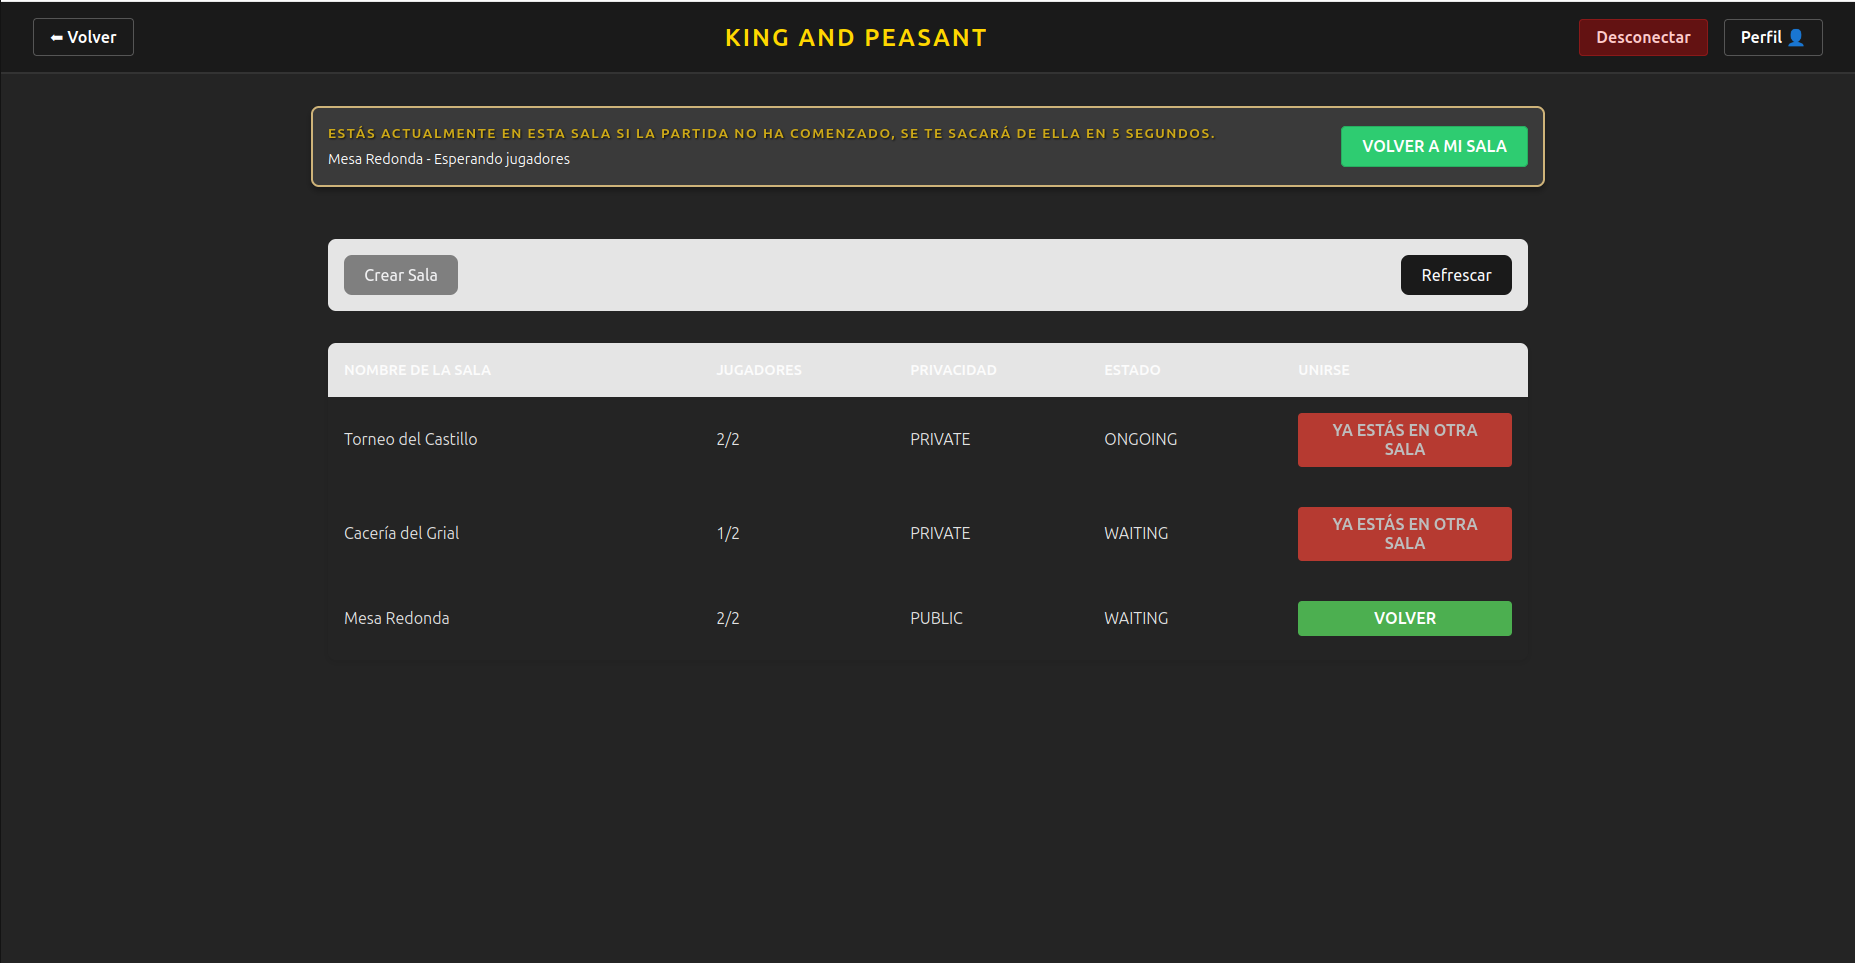
\includegraphics[width=\textwidth]{figures/manual/Volver a Sala.png}
\caption{Pantalla de Listado de Salas: Volver a la Sala}
\label{fig:Manual06}
\end{center}
\end{figure}

Tal y como detalla la Figura \ref{fig:Manual06}, si intentamos navegar por el menú mientras ya estamos dentro de una sala activa, el sistema nos alertará. Aparecerá un recuadro destacado con borde dorado en la parte superior advirtiendo que seremos expulsados de la sala en un plazo de 5 segundos si no regresamos. Para evitarlo, disponemos de un botón verde de \textit{Volver a mi sala} en ese mismo recuadro, o bien usando el botón de \textit{Volver} en la fila correspondiente de la tabla de salas.

\section{Sala}
\label{sec:sala}

\begin{figure}[H]
\begin{center}
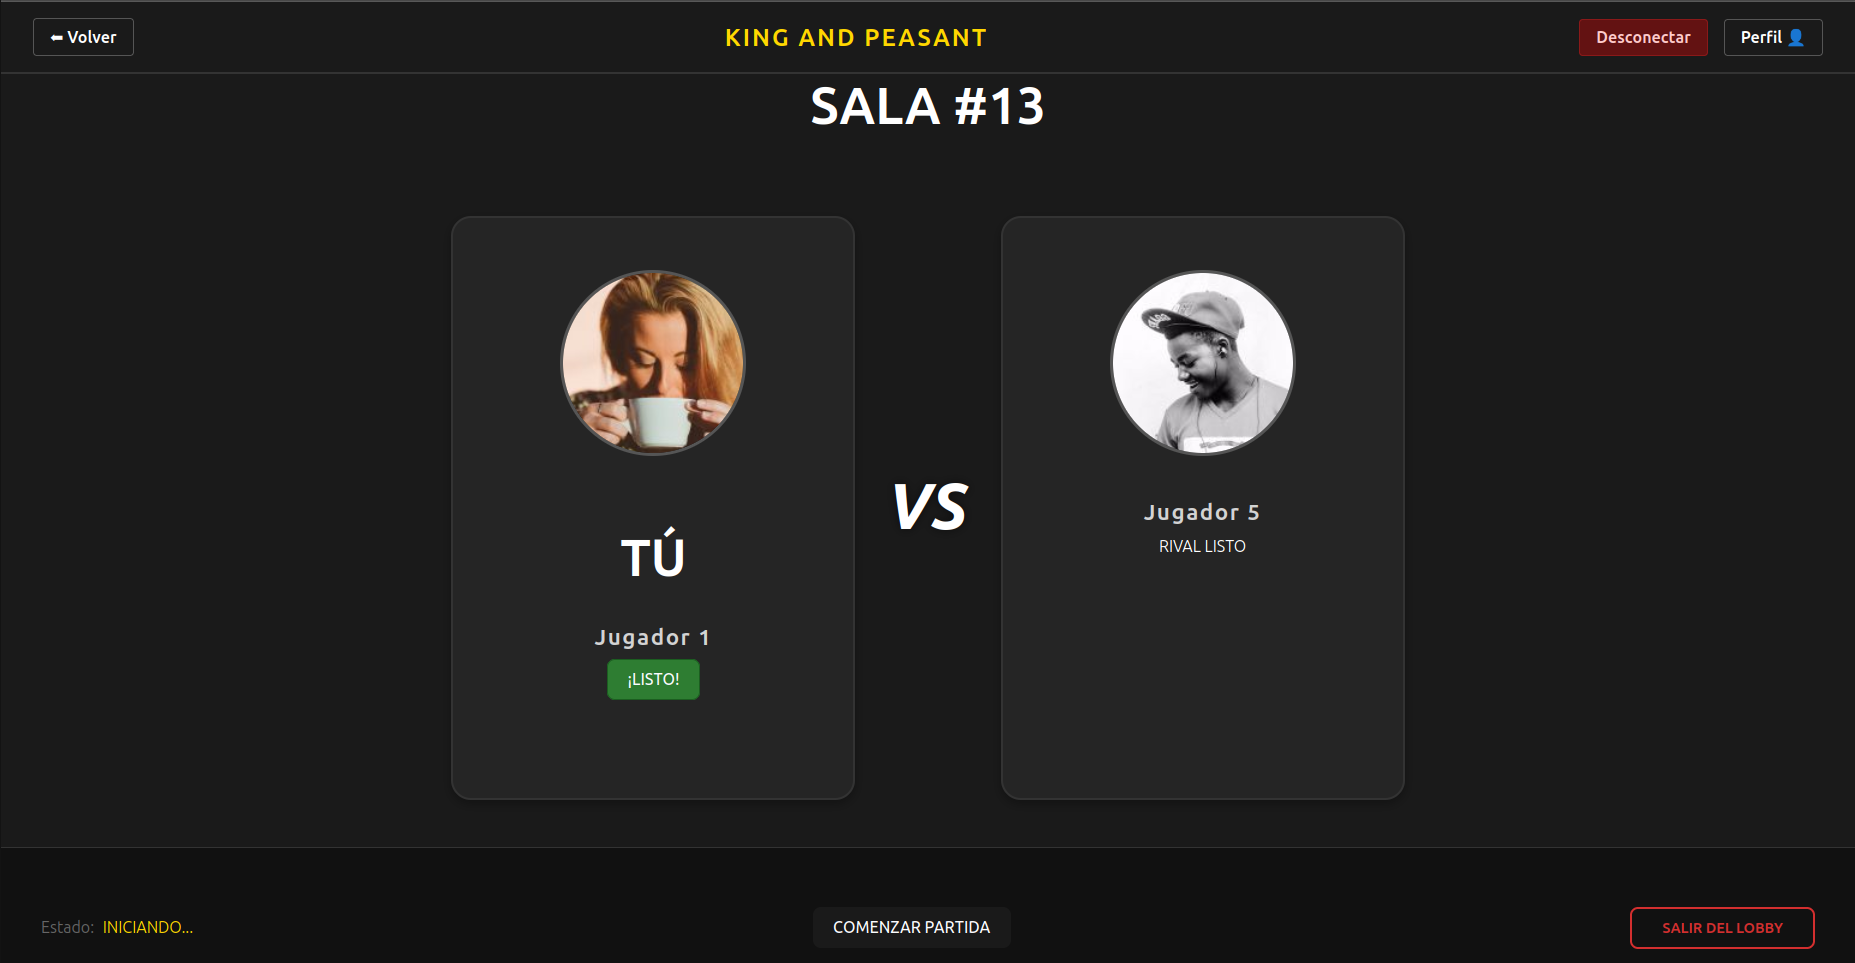
\includegraphics[width=\textwidth]{figures/manual/Sala.png}
\caption{Pantalla de Sala}
\label{fig:Manual07}
\end{center}
\end{figure}

En la Figura \ref{fig:Manual07} se expone la interfaz sala de espera previa a la partida. La pantalla muestra visualmente un enfrentamiento directo, colocando el avatar y nombre de nuestro usuario a la izquierda y los de nuestro oponente a la derecha, separados por un contundente ``VS''. 

Una vez dentro, es imperativo que marquemos el botón de \textit{¡Listo!} (ubicado bajo nuestro nombre) para confirmar nuestra disponibilidad. Cuando el sistema detecte que el texto ``Rival Listo'' aparece en el lado del oponente y nosotros también estamos preparados, el botón inferior de \textit{Comenzar Partida} se habilitará para que el creador de la sala inicie el juego. Si por algún motivo deseamos abandonar el enfrentamiento, podemos usar el botón rojo inferior derecho de \textit{Salir del Lobby}, lo que nos devolverá al listado de salas.

\section{Partida}
\label{sec:partida}

\subsection{Interfaz del Juego}
\begin{description}
    \item \textbf{Tu Área:}

    \begin{figure}[H]
    \begin{center}
    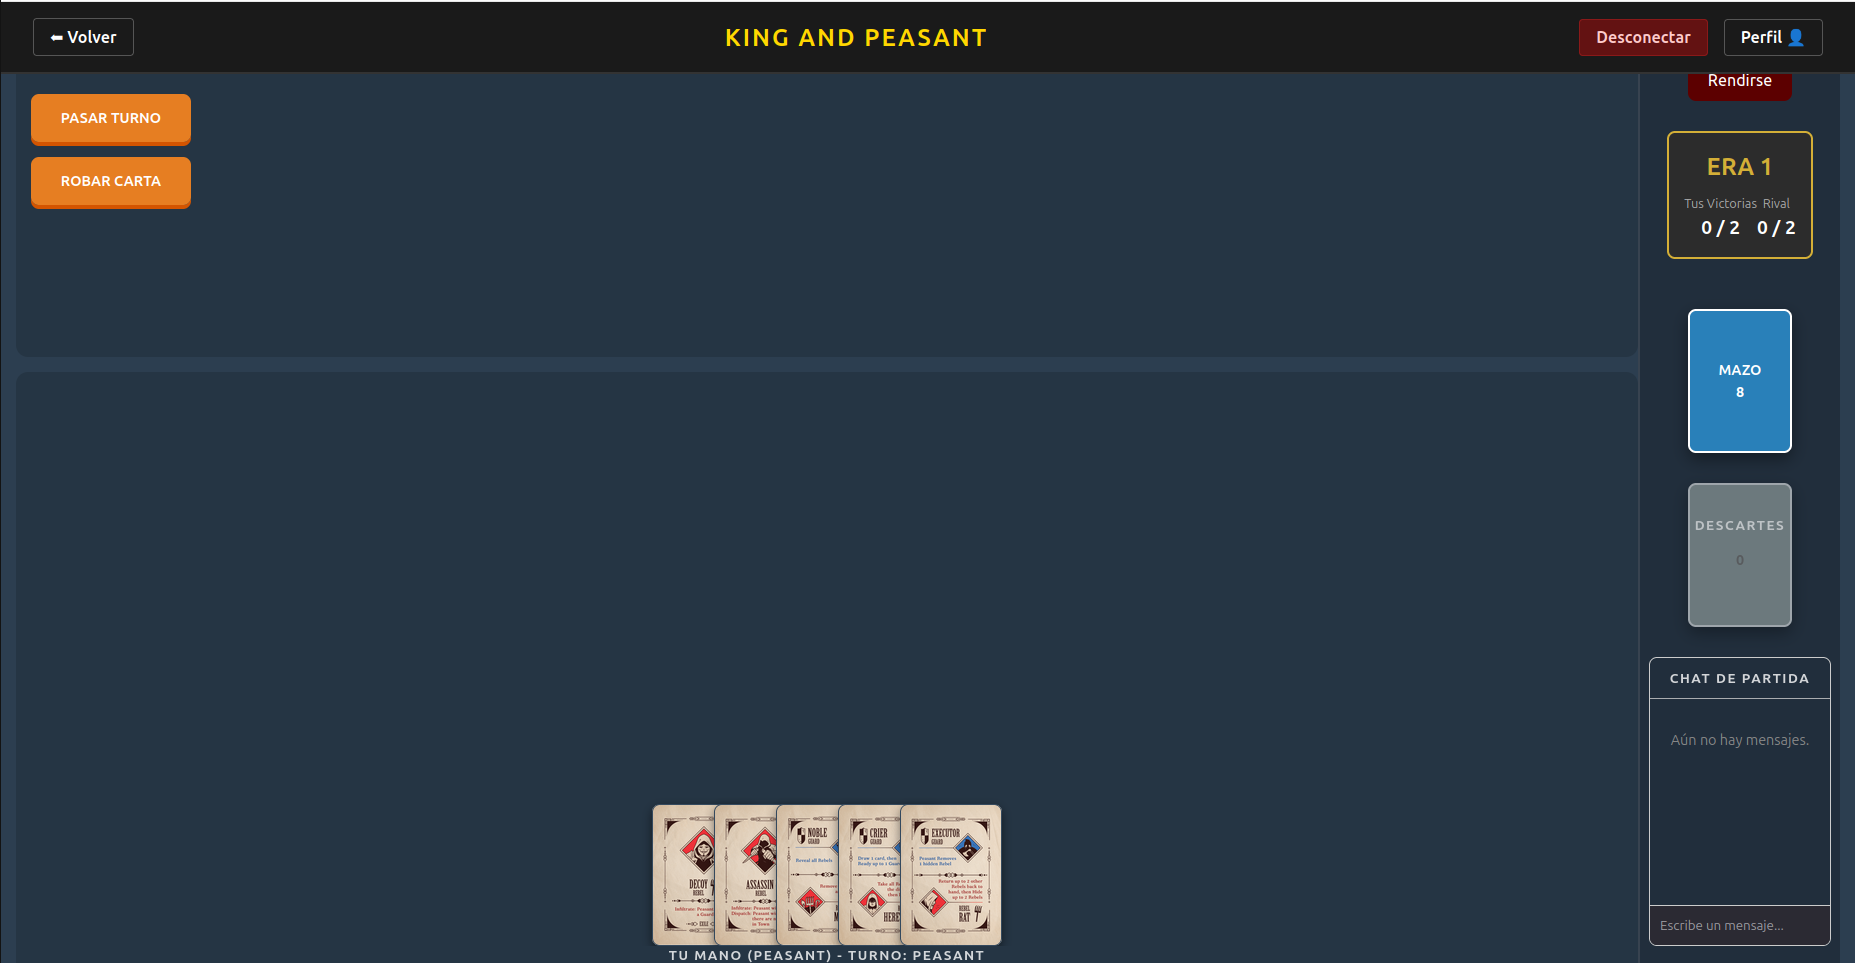
\includegraphics[width=\textwidth]{figures/manual/Partida Tu Mano.png}
    \caption{Pantalla de Partida: Tu Área}
    \label{fig:Manual08}
    \end{center}
    \end{figure}

    La Figura \ref{fig:Manual08} muestra la perspectiva inferior del tablero correspondiente a nuestro control. En la parte central inferior se despliegan boca arriba las cartas que conforman nuestra mano actual. Justo debajo de ellas, un indicador de texto nos recuerda en todo momento nuestro rol y de quién es el turno (por ejemplo: \textit{Tu mano (Peasant) - Turno: Peasant}). Sobre nuestra mano se extiende nuestro territorio del pueblo, la zona designada para colocar estratégicamente nuestras unidades durante el desarrollo del juego. 

    \item \textbf{Área del Rival:}

    \begin{figure}[H]
    \begin{center}
    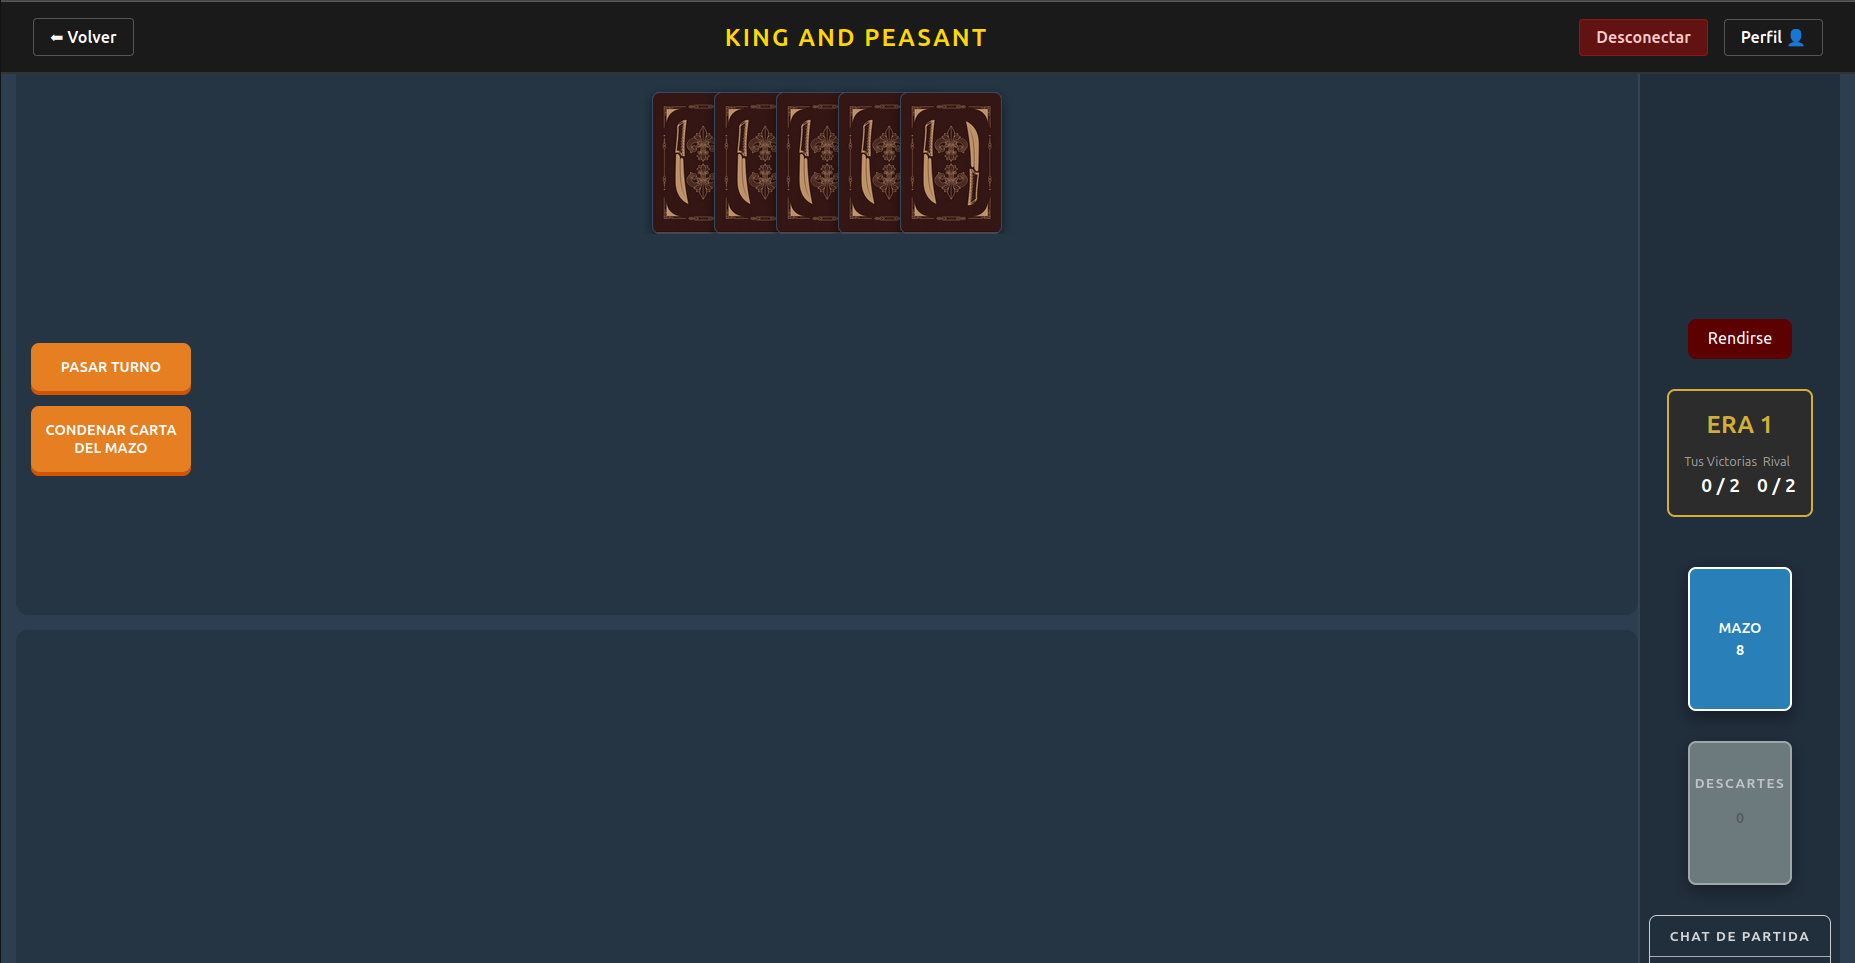
\includegraphics[width=\textwidth]{figures/manual/Partida Mano Rival.png}
    \caption{Pantalla de Partida: Área del Rival}
    \label{fig:Manual09}
    \end{center}
    \end{figure}

    En la Figura \ref{fig:Manual09} se ilustra la mitad superior de la pantalla, dedicada al oponente. En el extremo superior se visualizan las cartas de su mano, las cuales permanecen boca abajo revelando únicamente su reverso. Bajo su mano se encuentra el territorio del pueblo rival. Las cartas que el adversario coloque aquí se mostrarán boca abajo si están ocultas, o boca arriba si han sido reveladas como consecuencia de las acciones de la partida.

    \item \textbf{Panel Lateral Izquierdo (Acciones):}
    
    A la izquierda del tablero principal (visibles en color naranja) se ubican los botones de acción rápida, cuyo contenido varía en función del turno y la situación. Acciones habituales como \textit{Pasar Turno}, \textit{Robar Carta} o \textit{Condenar Carta del Mazo} aparecerán en esta columna para ser ejecutadas ágilmente.

    \item \textbf{Panel Lateral Derecho (Estado y Comunicación):}
    
    En la franja derecha se agrupa la información global de la partida. Arriba encontramos un botón rojo para \textit{Rendirse}, seguido de un marcador que indica la ronda actual (\textit{Era 1}) y el conteo de victorias de ambos jugadores. Debajo de esto se sitúan dos botones grandes: el mazo principal en color azul (indicando cuántas cartas restan por robar) y la pila de descartes en color gris. En la zona inferior derecha disponemos de una caja de chat en vivo para comunicarnos con nuestro rival.
\end{description}

\subsection{Acciones de Turno}

Durante tu turno, podrás interactuar con la interfaz para realizar diversas acciones dependiendo de tu rol estratégico (Rey o Campesino) y del estado del tablero:

\begin{description}

    \item \textbf{Robar Carta:}

    Pulsando el botón naranja correspondiente en el menú izquierdo, extraerás la primera carta del mazo para añadirla a tu mano.

    \item \textbf{Colocar Carta en Pueblo:}

    Haciendo clic sobre una carta de tipo \texttt{Guard} o \texttt{Rebel} en tu mano, la trasladarás a tu zona del pueblo en el tablero.

    \item \textbf{Jugar Carta en el Pueblo:}

    Selecciona una carta del pueblo para jugar su acción. En caso de que tu rol sea el de Campesino, solo puedes jugar cartas no reveladas.

    Si la carta se puede infiltrar, deberás seleccionarla y elegir la posición del mazo de forma interactiva donde quieres infiltrar la carta.

    \item \textbf{Jugar Acción:}

    Si seleccionas una carta de tipo \texttt{ACTION} directamente desde tu mano, su efecto se aplicará de inmediato y la carta irá a los descartes, sin necesidad de transitar previamente por el pueblo.

    \item \textbf{Pasar Turno:}

    Utilizando el botón naranja de \textit{Pasar Turno} ubicado en la columna izquierda, finalizarás tus acciones y cederás el control al adversario.

    \item \textbf{Condenar Rebelde:}

    Si juegas bajo el rol del Rey, la interfaz te habilitará la opción letal de condenar a un rebelde no revelado. Puedes ejecutar esto haciendo clic directo sobre una carta oculta en el pueblo rival, o usando el botón \textit{Condenar Carta del Mazo} del panel izquierdo para ejecutar la carta superior del mazo. 

    \texttt{CUIDADO: Esta acción es definitiva. Culminará inmediatamente en victoria o derrota para el Rey dependiendo de si la carta ejecutada resulta ser el Asesino.}

    \item \textbf{Acciones Pendientes:}

    El flujo normal del juego puede verse interrumpido cuando una carta jugada por tu rival requiera tu intervención obligatoria (por ejemplo, seleccionar un objetivo válido). La interfaz central te exigirá tomar una decisión y seleccionar una respuesta válida antes de permitirte continuar con otras acciones.
\end{description}

\section{Fin de la Era y Fin de la Partida}
\label{sec:fin_partida}

Una vez que se cumplen las condiciones de victoria específicas de alguno de los dos roles, el tablero se bloquea y aparece una pantalla modal anunciando al ganador de la ronda actual. Este cuadro ofrece un resumen estadístico rápido de la Era finalizada y contiene un botón de confirmación que ambos jugadores deben pulsar para proceder a la siguiente ronda.

El sistema lleva el registro acumulativo en el panel lateral. En el momento en que un jugador logre alzarse con la victoria en dos Eras distintas, el juego declarará el final definitivo de la partida y la interfaz redirigirá automáticamente a ambos usuarios de vuelta a la sala de espera original.
